\section{Data Placement}

\subsection{Object Address}

\begin{frame}{Object Addressing}
    \begin{figure}[htpb]
        \centering
        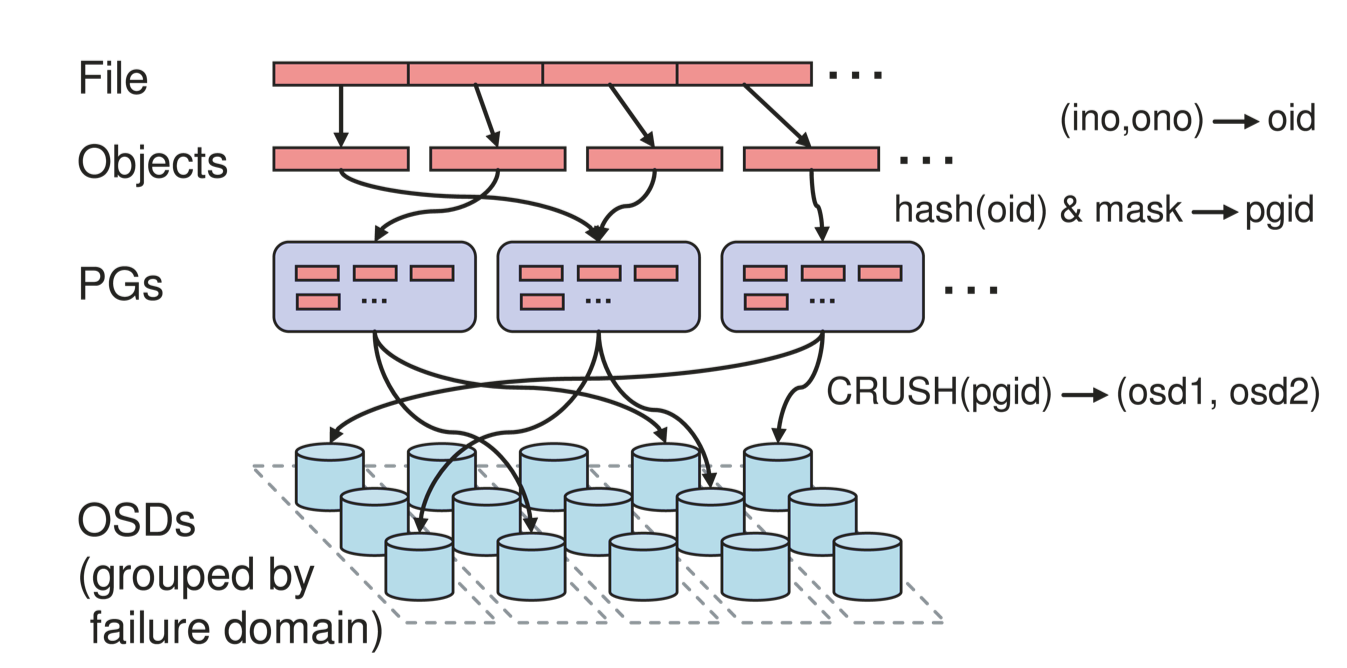
\includegraphics[width=0.8\linewidth]{data-distribution.png}
    \end{figure}
\end{frame}

\begin{frame}{寻址流程}
    \begin{itemize}
        \item \textbf{File -> Object}
            \begin{itemize}
                \item 将用户要操作的File,映射成RADOS能够处理的Object
                \item 本质上是按照Object的最大Size对File进行切分
                \item 切分可以使大小不限的File变成最大Size一致、可以被RADOS高效管理的Object
                \item 切分同时也可以让对单一File实施的串行处理变成对多个Object实施的并行化处理
            \end{itemize}
        \item \textbf{Object -> PG}
            \begin{itemize}
                \item 将每个Object独立的映射到一个PG中去
                \item 固定的Hash算法
            \end{itemize}
        \item \textbf{PG -> OSD}
            \begin{itemize}
                \item 将作为Object的逻辑组织单元的PG映射到数据的实际存储单元OSD
                \item 采用CRUSH算法
            \end{itemize}
    \end{itemize}
\end{frame}

\begin{frame}{CRUSH Function}
    \begin{figure}[htpb]
        \centering
        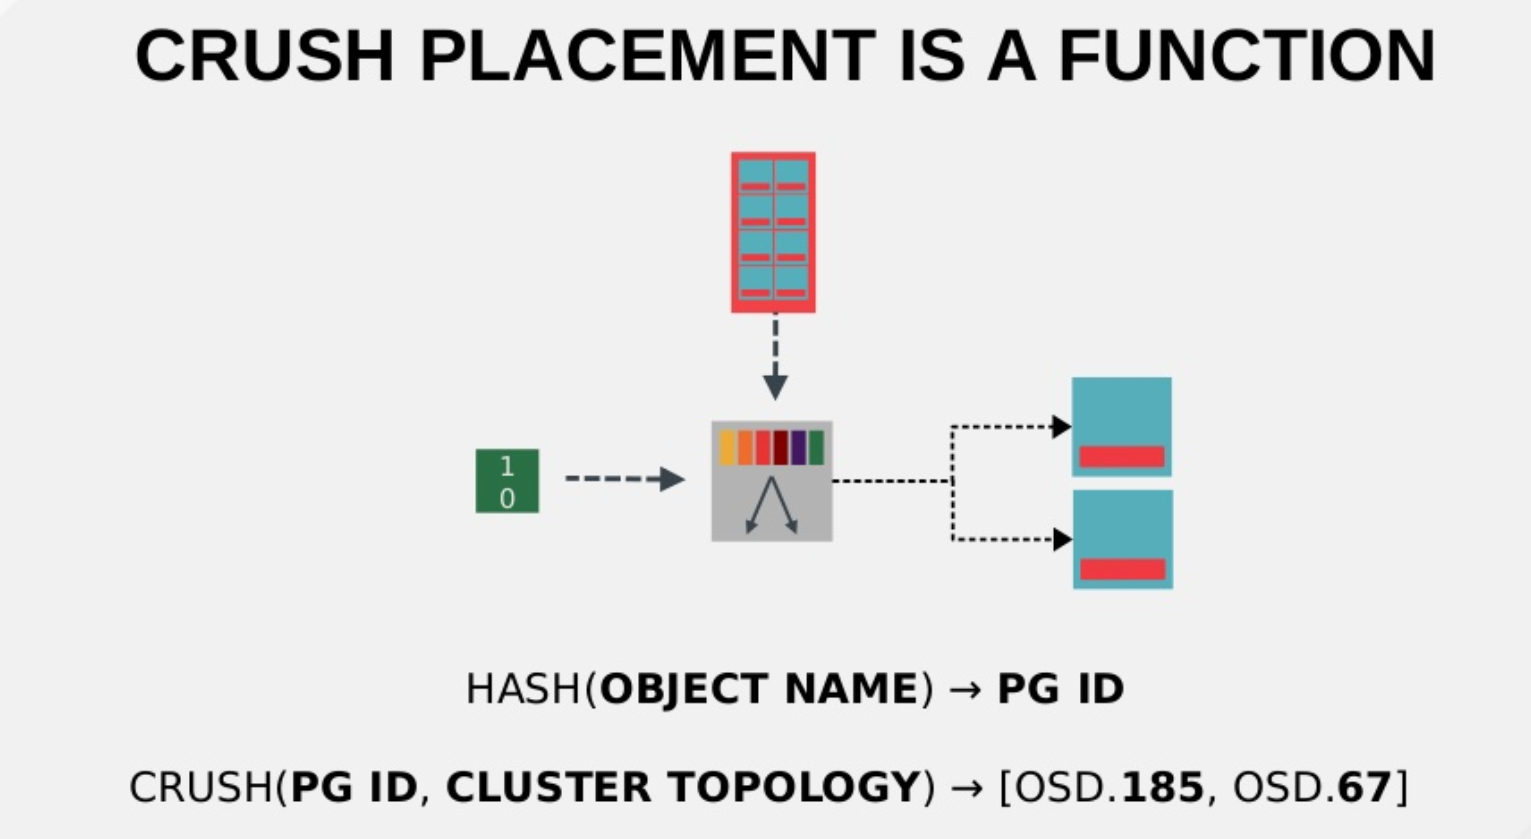
\includegraphics[width=0.9\linewidth]{crush-function.png}
    \end{figure}
\end{frame}

\begin{frame}{CRUSH}
    \begin{itemize}
        \item CRUSH(x) -> ($osd_{n1}, osd_{n2}, osd_{n3}$)
            \begin{itemize}
                \item Inputs
                    \begin{itemize}
                        \item x is the placement group
                        \item hierarchical cluster map
                        \item placement rules
                    \end{itemize}
                \item Outputs: a list of OSDs
            \end{itemize}
        \item Advantages
            \begin{itemize}
                \item Anyone can calculate object location
                \item Cluster map infrequently updated
            \end{itemize}
    \end{itemize}
\end{frame}

\begin{frame}{CRUSH}
    \begin{figure}[htpb]
        \centering
        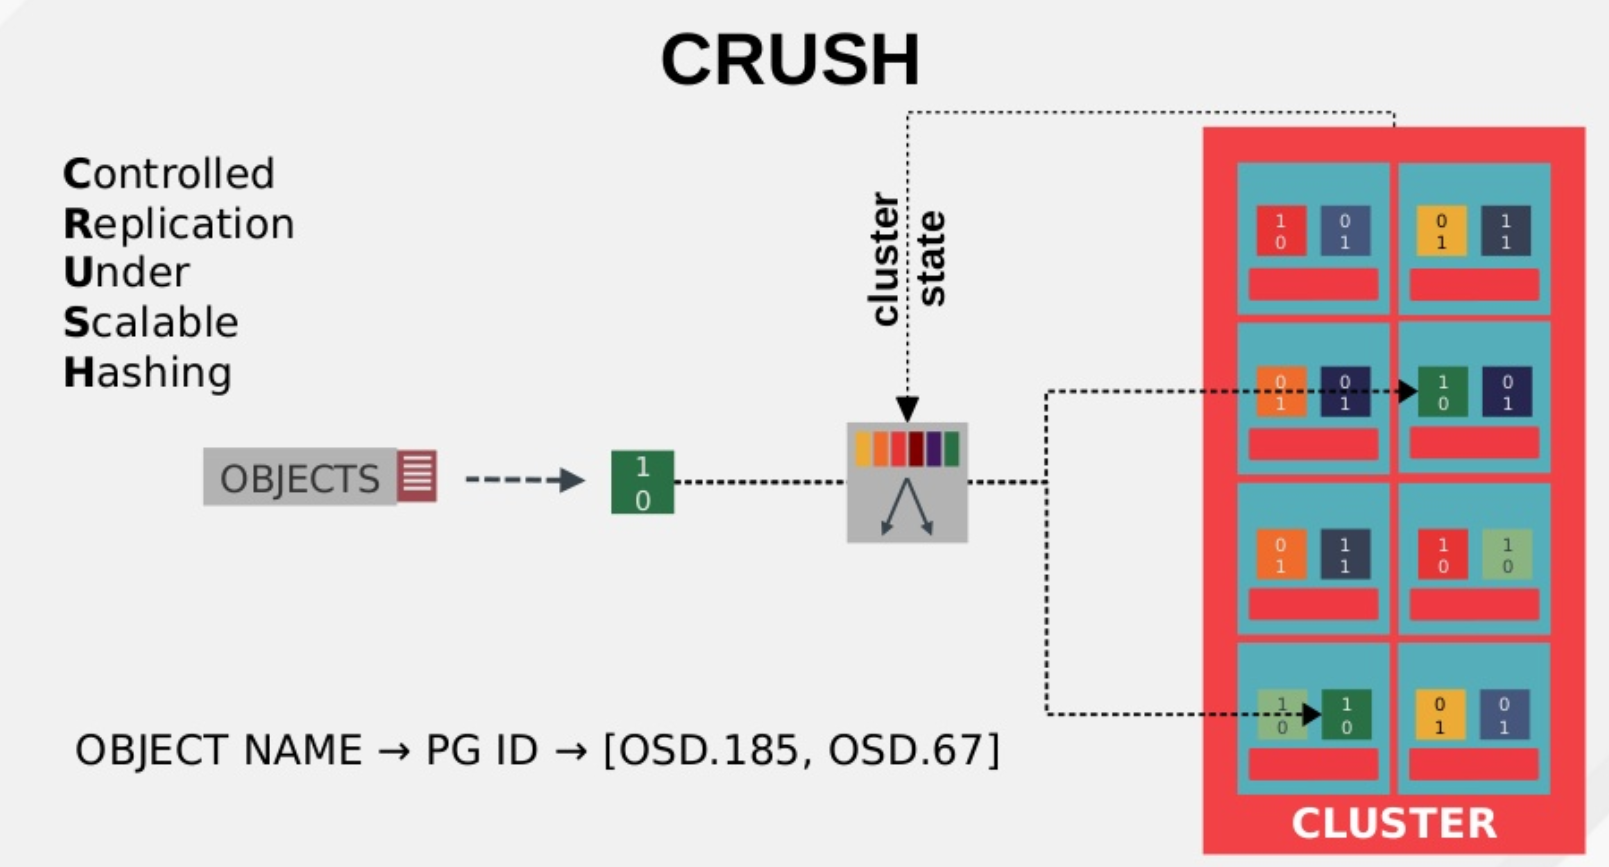
\includegraphics[width=0.9\linewidth]{crush.png}
    \end{figure}
\end{frame}

\begin{frame}{CRUSH}
    CRUSH(Controlled Replication Under Scalable Hashing)
    \begin{itemize}
        \item \textbf{Ceph's data distribution mechanism}
        \item \textbf{Pseudo-random placement algorithm}
            \begin{itemize}
                \item Deterministic function of inputs
                \item Clients can compute data location
            \end{itemize}
        \item \textbf{Rule-based configuration}
            \begin{itemize}
                \item Desired/required replica count
                \item Affinity/distribution rules
                \item Infrastructure topology
                \item Weighting
            \end{itemize}
        \item \textbf{Excellent data distribution}
            \begin{itemize}
                \item De-clustered placement
                \item Excellent data-re-distribution
                %\item Migration proportional to change
            \end{itemize}
    \end{itemize}
\end{frame}

\begin{frame}{Key CRUSH Properties}
    \begin{itemize}
        \item \textbf{No Storage} - Only need to know the cluster topology
        \item \textbf{Fast} - microseconds, even for very large clusters
        \item \textbf{Stable} - very little data movement when topology changes
        \item \textbf{Reliable} - placement is constrained by \textbf{\textit{failure domains}}
        \item \textbf{Flexible} - replication, erasure codes, complex placement schemes
    \end{itemize}
\end{frame}

\subsection{Cluster Map}

%\begin{frame}{CRUSH Map Hierarchy}
%    \begin{itemize}
%        \item \textbf{Device list: List of OSDs}
%        \item \textbf{Buckets: Hierarchical aggregation of storage locations}
%            \begin{itemize}
%                \item Buckets have an assigned weight
%                \item Buckets have a type
%                    \begin{itemize}
%                        \item root
%                        \item datacenter
%                        \item rack
%                        \item host
%                        \item osd
%                    \end{itemize}
%            \end{itemize}
%        \item \textbf{Rules: define data placement for pools}
%    \end{itemize}
%\end{frame}
%
%\begin{frame}{CRUSH Map Hierarchy}
%    The CRUSH Map contains
%    \begin{itemize}
%        \item A list of OSDs
%        \item A list of the rules to tell CRUSH how data is to be replicated
%        \item A default CRUSH is created where you create the cluster
%    \end{itemize}
%\end{frame}

\begin{frame}{Hierarchical Cluster Map}
    \begin{itemize}
        \item \textbf{The cluster map is composed of \textit{device} and \textit{bucket}}
        \begin{itemize}
            \item \textbf{device}: basic storage device, OSD
            \item \textbf{bucket}: container, and contain any number of devices or other buckets
            \item \textbf{item}: member of bucket, can be device or lower level bucket
            \item both device and bucket have numerical identifiers and weight values associated with them
        \end{itemize}
        \item bucket type:
            \begin{itemize}
                \item root, region, datacenter, room, row, rack, host
                \item you can define your own bucket type and hierarchy relation
            \end{itemize}
    \end{itemize}
\end{frame}

\begin{frame}[fragile]{Hierarchical Cluster Map}
    \begin{columns}
        \begin{column}{0.35\textwidth}
\begin{lstlisting}[language=python]
# devices
device 0 osd.0 class hdd
device 1 osd.1 class hdd
device 2 osd.2 class hdd
device 3 osd.3 class hdd
\end{lstlisting}

\begin{lstlisting}[language=python]
# buckets
host node1 {
    id -2
    id -3 class hdd
    # weight 1.000
    alg straw2
    hash 0    # rjenkins1
    item osd.0 weight 1.000
}
\end{lstlisting}
\begin{lstlisting}[language=python]
host node2 {
    id -5
    id -6 class hdd
    # weight 1.000
    alg straw2
    hash 0    # rjenkins1
    item osd.1 weight 1.000
}
\end{lstlisting}
        \end{column}
        \begin{column}{0.55\textwidth}
            
\begin{lstlisting}[language=python]
host node3 {
    id -7
    id -8 class hdd
    # weight 2.000
    alg straw2
    hash 0    # rjenkins1
    item osd.2 weight 1.000
    item osd.3 weight 1.000
}
\end{lstlisting}

\begin{lstlisting}[language=python]
root default {
    id -1   # bucket id, 一般为负数
    # weight 4.000 # sum of item's weight
    alg straw2 # algorithm for random select
    hash 0    # rjenkins1 # hash function type
    item node1 weight 1.000
    item node2 weight 1.000
    item node3 weight 2.000
}
\end{lstlisting}
        \end{column}
    \end{columns}
\end{frame}

\begin{frame}{Cluster Map Example}
    \begin{figure}[htpb]
        \centering
        \includegraphics[width=0.7\linewidth]{crush-cluster-map.png}
    \end{figure}
\end{frame}

\begin{frame}{Failure Domains}
    \begin{itemize}
        \item \textbf{CRUSH generates \textit{n} distinct target devices(OSDs)}
            \begin{itemize}
                \item may be replicas or erasure coding shards
            \end{itemize}
        \item \textbf{Separate replicas across failure domains}
            \begin{itemize}
                \item single failure should only compromise one replica
                \item size of failure domain depends on cluster size
                    \begin{itemize}
                        \item disk
                        \item host(NIC, RAM, PS)
                        \item rack(ToR switch)
                        \item row(distribution switch, ...)
                        \item data center(eletricity...)
                    \end{itemize}
                \item based on types in CRUSH hierarchy
            \end{itemize}
        %\item Sources of failure should be aligned
        %    \begin{itemize}
        %        \item per-rack switch and PDU and physical location
        %    \end{itemize}
    \end{itemize}
\end{frame}

\subsection{Placement Rule}


\begin{frame}[fragile]{CRUSH Rules}
    \begin{columns}
        \begin{column}{0.6\textwidth}
            \begin{itemize}
                \item \textbf{Policy}
                    \begin{itemize}
                        \item where to place replicas
                        \item the failure domain
                    \end{itemize}
                \item \textbf{Trivial program}
                    \begin{itemize}
                        \item short sequence of imperative commands
                        \item flexible, extensible
                        \item not particularly nice for humans
                    \end{itemize}
            \end{itemize} 
        \end{column}
        \begin{column}{0.4\textwidth}
\begin{lstlisting}[language=python]
rule flat {
    ruleset 0   # ruleset id
    type replicated
    min_size 1  # 副本最小数量
    max_size 10 # 副本最大数量
    step take root
    step choose fistn 0 type osd
    step emit
}
\end{lstlisting}
       \end{column}
   \end{columns} 
\end{frame}

\begin{frame}{Basic Operation: Step}
    \begin{itemize}
        \item \textbf{take}: choose a bucket(often root bucket)
        \item \textbf{choose}
            \begin{itemize}
                \item \textbf{choose firstn \{num\} type \{bucket-type\}}
                    \begin{itemize}
                        \item 选择num个bucket-type的item
                    \end{itemize}
                \item \textbf{chooseleaf firstn \{num\} type \{bucket-type\}}
                    \begin{itemize}
                        \item 先选择bucket-type类型的item,再递归选择叶子节点的OSD
                    \end{itemize}
                \item meaning of num parameter
                    \begin{itemize}
                        \item if $num == 0$, choose pool-num-replicas buckets(all available)
                        \item if $num > 0 and < pool-num-replicas$, choose that many buckets
                        \item if $num < 0$, it means $pool-num-replicas - num$
                    \end{itemize}
            \end{itemize}
        \item \textbf{emit} 
    \end{itemize} 
\end{frame}

\begin{frame}[fragile]{RuleSet}
\begin{lstlisting}[language=python]
rule replicated_ruleset {
    ruleset 0       # ruleset id
    type replicated # type replicated or erasure code

    min_size 1
    max_size 10

    step take root
    step choose firstn 1 type row
    step choose firstn 3 type cabinet
    step choose firstn 1 type osd
    step emit
}
\end{lstlisting}
\end{frame}

\begin{frame}{CRUSH Rules}
    \begin{figure}[htpb]
        \centering
        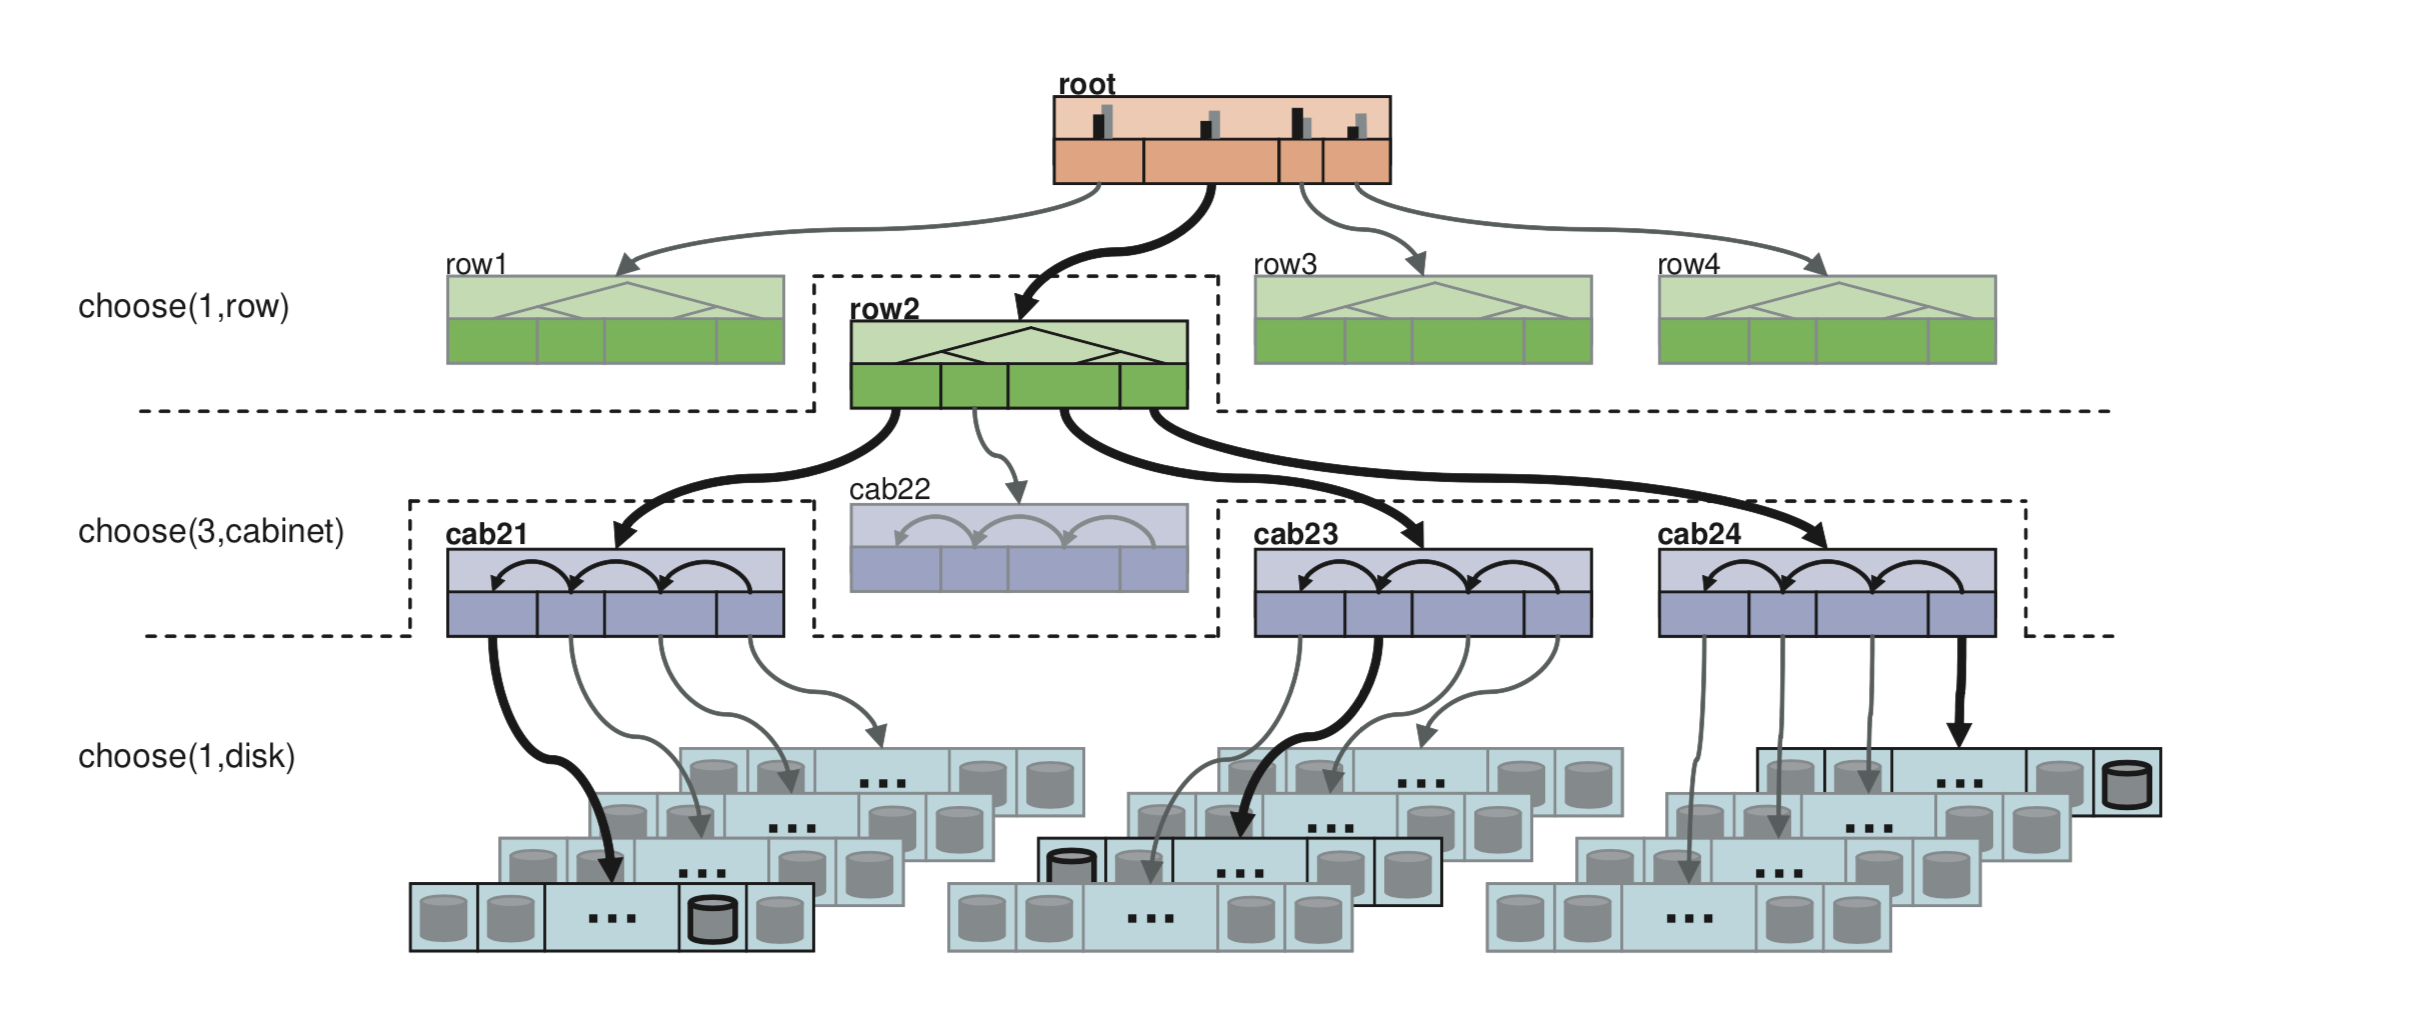
\includegraphics[width=1\linewidth]{crush-ruleset.png}
    \end{figure}
\end{frame}

\begin{frame}[fragile]{RuleSet Example}
\begin{lstlisting}[language=python]
rule ssd-primary {
    ruleset 5       # ruleset id
    type replicated # type replicated or erasure code

    min_size 5
    max_size 10

    step take ssd   # 选择ssd这个root bucket作为输入
    step chooseleaf firstn 1 type host   # 选择一个host,再递归选择叶子节点的osd
    step emit

    step take hdd   # 选择hdd这个root bucket作为输入
    step chooseleaf firstn -1 type host   # 选择总副本数减一个host,再递归选择叶子节点的osd
    step emit
}
\end{lstlisting}
\end{frame}

\begin{frame}{Bucket Algorithms}
    \begin{itemize}
        \item \textbf{Goal of CRUSH algorithm}
            \begin{itemize}
                \item efficiency and scalability of the mapping algorithm
                \item minimum data migration to restore a balanced distribution when the cluster changes due to the addition or removal of devices.
            \end{itemize}
        \item \textbf{CRUSH define 4 kinds of buckets to represent internal nodes in the cluster hierarchy}
            \begin{itemize}
                \item uniform buckets
                \item list buckets
                \item tree buckets
                \item straw buckets
            \end{itemize}
        \item Each bucket type is based on a \textbf{different internal data structure} and utilizes a \textbf{different function c(r, x) for pseudo-randomly choosing nested items} during the replica placement process
        \item Each bucket type represents a different \textbf{tradeoff between computation and reorganization efficiency}
    \end{itemize}
\end{frame}

\begin{frame}{How does it work?}
    \begin{figure}[htpb]
        \centering
        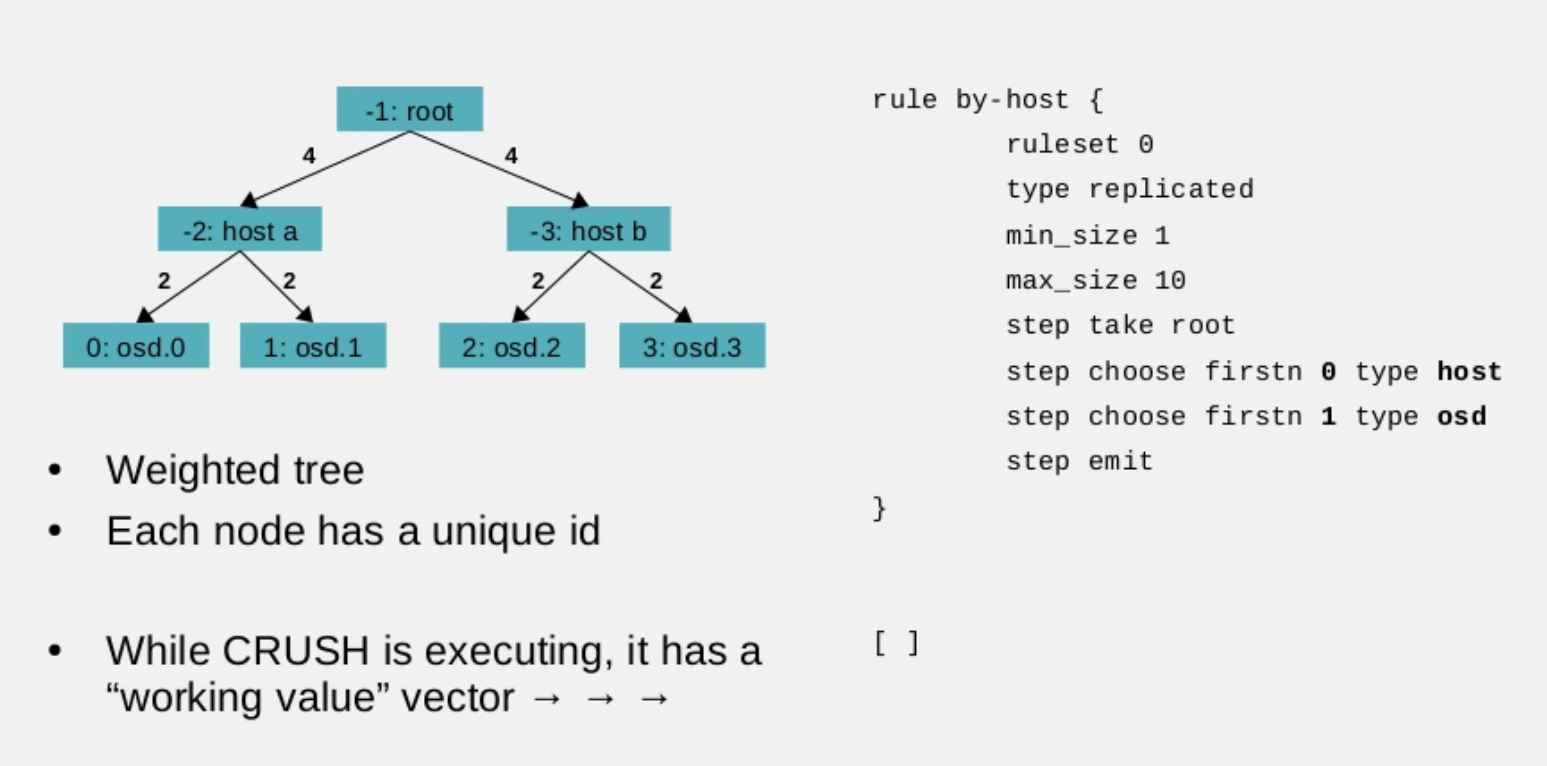
\includegraphics[width=0.8\linewidth]{crush0.png}
    \end{figure}
\end{frame}

\begin{frame}{How does it work?}
    \begin{figure}[htpb]
        \centering
        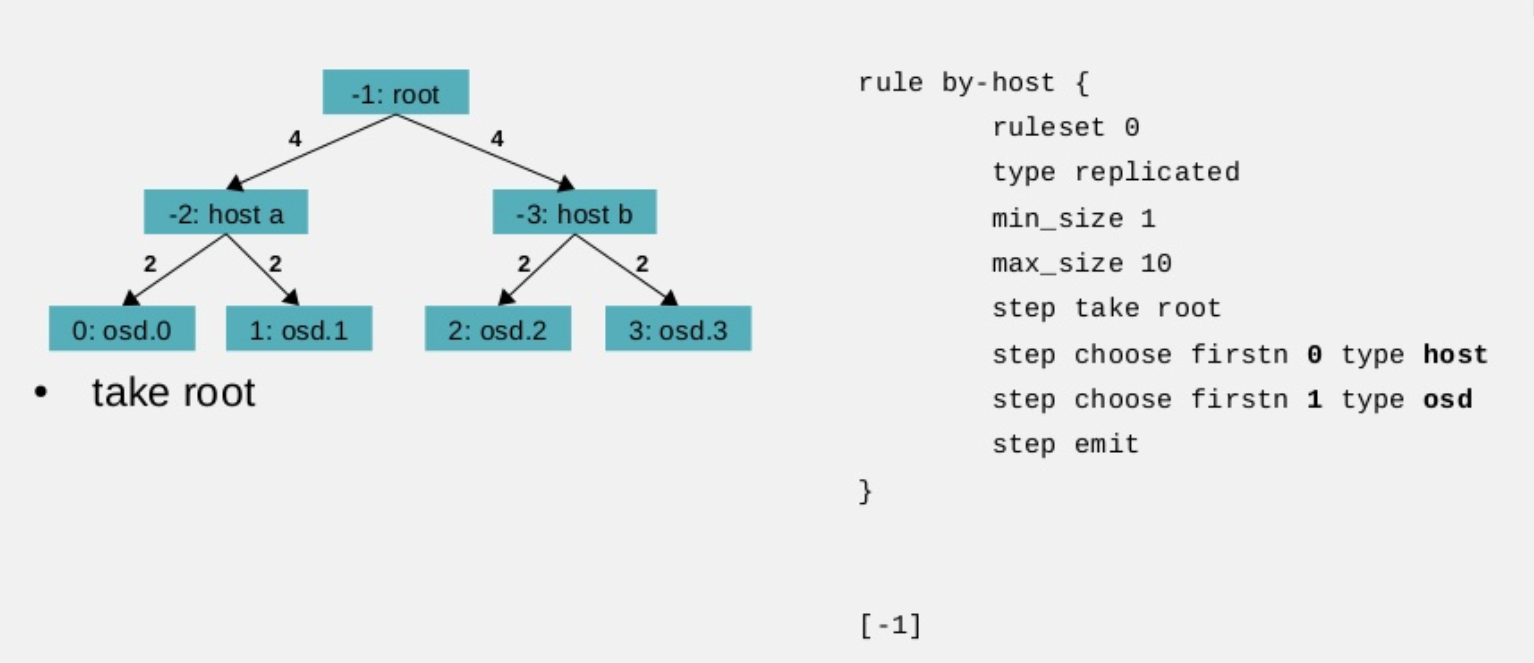
\includegraphics[width=0.8\linewidth]{crush1.png}
    \end{figure}
\end{frame}

\begin{frame}{How does it work?}
    \begin{figure}[htpb]
        \centering
        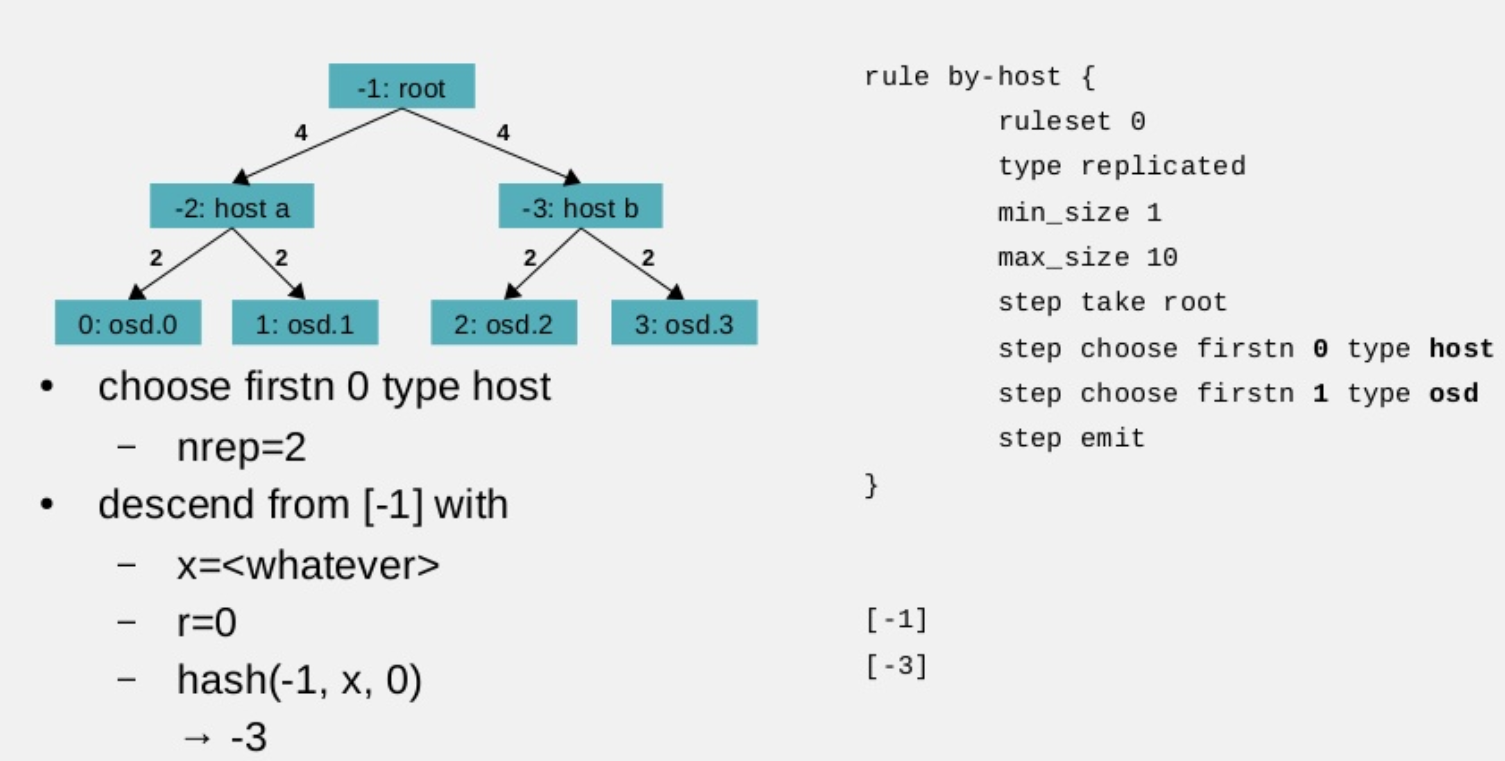
\includegraphics[width=0.8\linewidth]{crush2.png}
    \end{figure}
\end{frame}

\begin{frame}{How does it work?}
    \begin{figure}[htpb]
        \centering
        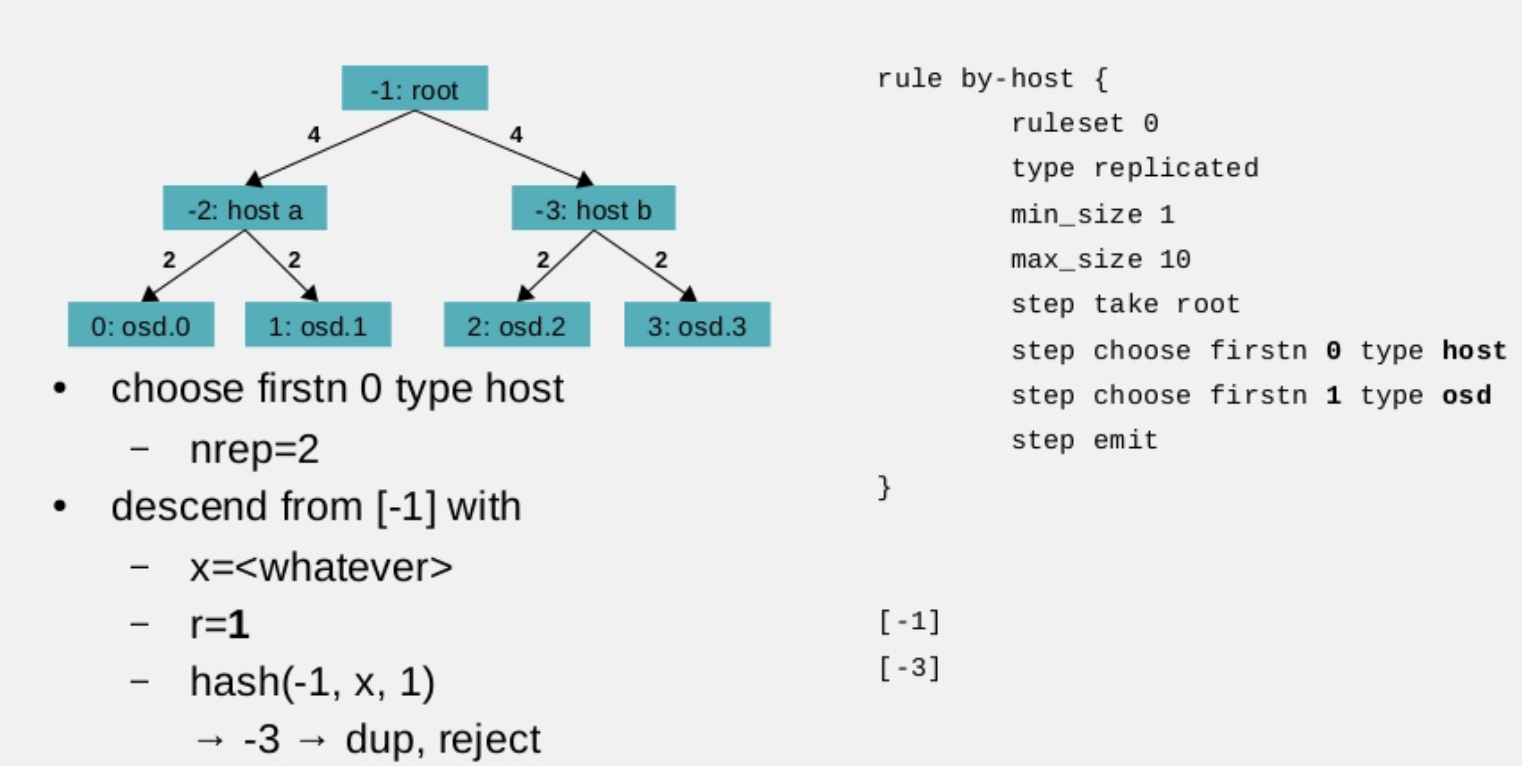
\includegraphics[width=0.8\linewidth]{crush3.png}
    \end{figure}
\end{frame}

\begin{frame}{How does it work?}
    \begin{figure}[htpb]
        \centering
        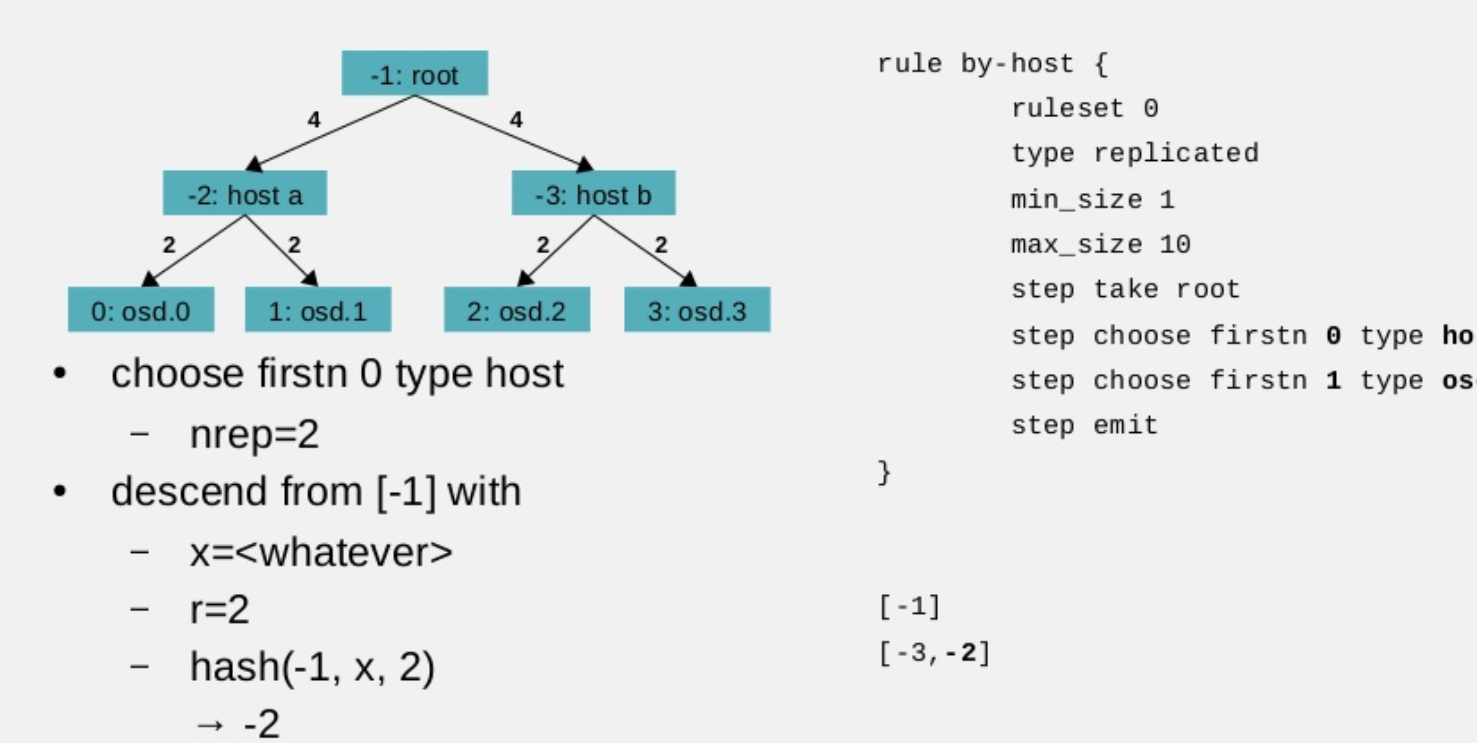
\includegraphics[width=0.8\linewidth]{crush4.png}
    \end{figure}
\end{frame}

\begin{frame}{How does it work?}
    \begin{figure}[htpb]
        \centering
        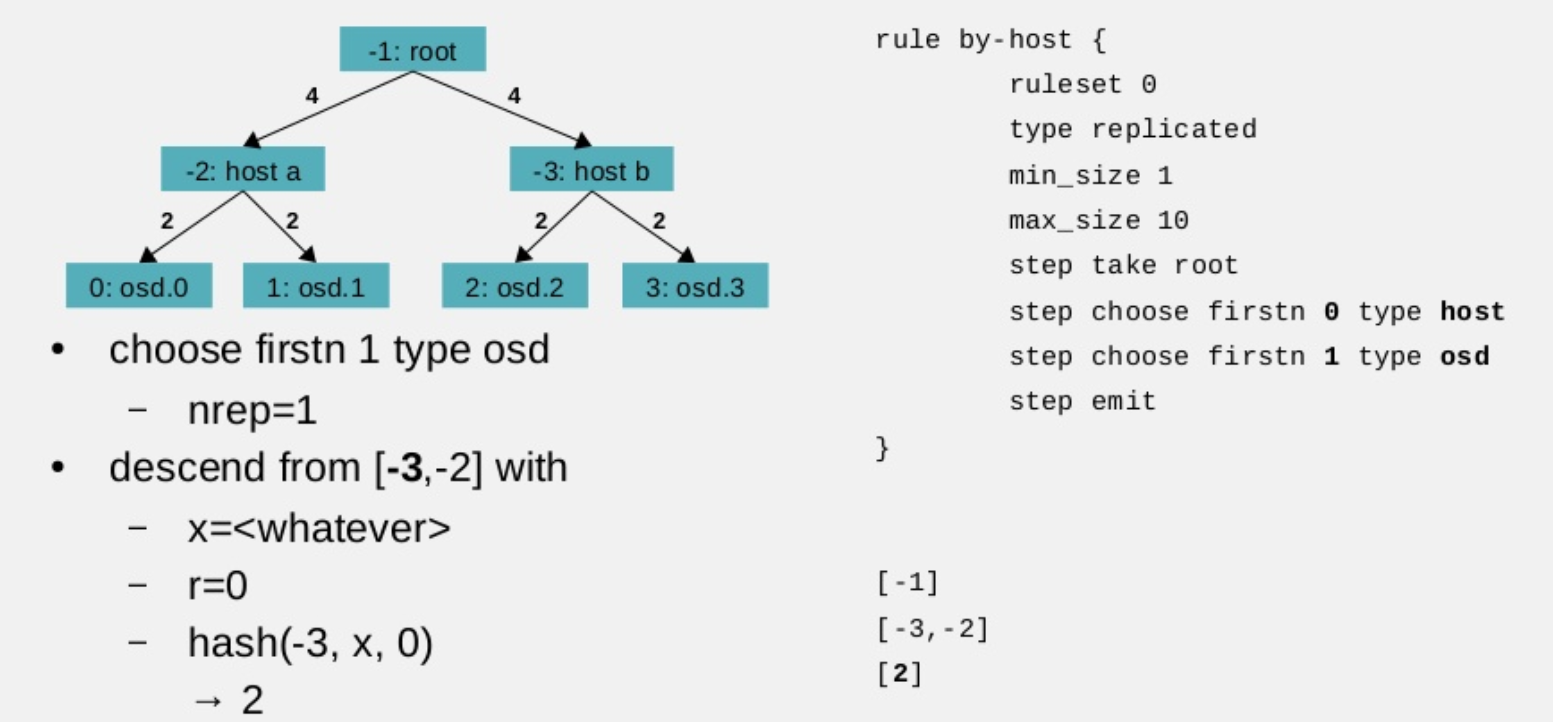
\includegraphics[width=0.8\linewidth]{crush5.png}
    \end{figure}
\end{frame}

\begin{frame}{How does it work?}
    \begin{figure}[htpb]
        \centering
        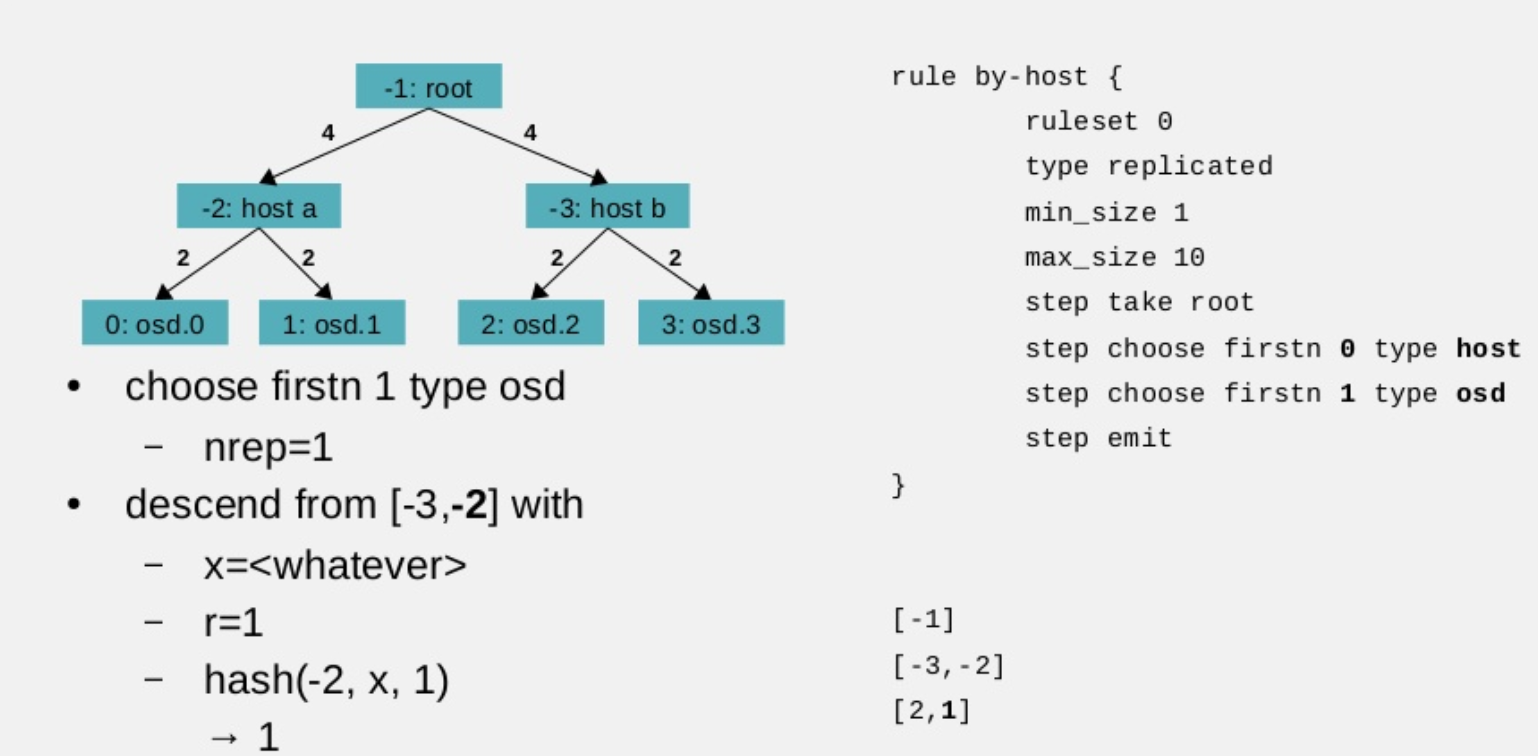
\includegraphics[width=0.8\linewidth]{crush6.png}
    \end{figure}
\end{frame}

\begin{frame}{Bucket Algorithms}
    \begin{itemize}
        \item \textbf{Many algorithms for selecting a child}
            \begin{itemize}
                \item every internal tree node has a type
                \item tradeof between time/computation and rebalancing behavior
                \item can mix types within a tree
            \end{itemize}
        \item \textbf{uniform}
            \begin{itemize}
                \item $hash(nodeid, x, r) \% num_children$
                \item fiexed $O(1)$ time
                \item addint child shuffles everything
            \end{itemize}
        \item \textbf{straw2}
            \begin{itemize}
                \item $hash(nodeid, x, r, child)$ for every child
                \item scale based on child weight
                \item pick the biggest value
                \item $O(n)$ time
            \end{itemize}
        \item \textbf{adding or removing child}
            \begin{itemize}
                \item only moves values to or from that child
                \item still fast enough for small n
            \end{itemize}
    \end{itemize}
\end{frame}

%\begin{frame}{Uniform Buckets}
%    
%\end{frame}

%\begin{frame}{List Buckets}
    
%\end{frame}

%\begin{frame}{Tree Buckets}
%    
%\end{frame}

%\begin{frame}{Straw Buckets}
%    
%\end{frame}

